\chapter{Weekly Progress}
\fix{}{Now, I think it would be good to have reflections for each part. For example now you plan to do a code-freeze - then would be a good spot to look back on your 
last weeks and reflect on your project working style - e.g., what would you do differently the next time etc - what would you do the same?
Maybe you can do 3-4 big reflections in total, with the last one  looking back over the whole project (that one a bit longer than the other ones)}
In this chapter our weekly progress and thoughts are described\ldots

\section*{Week 37}
\subsection*{What Happend This Week}
To start with the project we researched upon our topic ``\fb'' and different
methods for gathering a vast amount of user data to identify a filter bubble. We
decided to check social media sites as a source for user data; we thought about
Facebook, Twitter and Reddit. We also investigated how to use the user data we
could potentially gather and what we would want and do with it. During our Web
Intelligence course, we learned about web crawlers, see section
\ref{subsec:crawler}, it is the method used by search engines to collect data.

We planned our workflow this semester, we are going to use some elements from
SCRUM to manage what has and have to be done and who works on the tasks. We set
up GIT repositories for code and report and split some responsibilities out
between our members, such as supervisor contact, repository and report.

\subsection*{Reflection}
We have found that social media sites were a suitable choice to gather a vast
amount of user information, which we reckon can be used to identify a \fb. We
are still in the initiating phase of the project so much can change. We decided
to write our report in Latex, using Eclipse as editor and GIT for versions control.
This is the style half the group have been doing, and it is causing minor
inconvenience for two group members adjusting to this. During this week we might
have used a little too much time discussing work preferences, it would
propably be better to list and discuss the advantages and disadvantages of the
choices.

\subsection*{Next Week}
During the next week, we would like to have a draft ready for the different
researched parts, from this week, ready for the report. Our supervisor sent some
links with useful information, these should be examined and noted upon depending
on usage. Moreover, we also want to define a description of the problem we try
to solve this semester.

%This week we have researched different social hubs, mainly Facebook and Twitter
% and some articles about how to place posts into categories on a topic; if
% people are for or against it. Description of web crawlers and explored some
% our possibilities for using it this semester. We have setup the work process
% for the semester, talked about the tools and methods we will be using to
% structure the project. 

%Mail: Couple of thoughts:
%Crawl social networks to get an idea of the expanse of the user’s filterbubble,
%by analysing the influences from contacts and pages they follow. This could
% also include an analysis of their likes and shares/retweets. In addition to this, we
%could compare with preexisting knowledge of news sources/sites.
%Given a website sift for keywords and look for sites where there is a
%concentration of these these words, this can be repeated a number of times,
% with the first website as the root.

%Ideas on how to start:
%Facebook has a lot of data available, along with an reasonable? API.
%Research webcrawlers
\section*{Week 38} \subsection*{What Happend This Week} 
This week we have researched further on social media sites and articles about
how to sort and learn using user data from social media sites. We have furthered
our knowledge on web crawlers and how one could use it this semester. In Web
Intelligence we have continued developing on the crawler, and it looks promising
for our project. We have evaluated on the tools we decided to use and how we
will be using them, we have decided to use a board and Trello to keep track of
task, with a member of the group in charge of keeping either updated. Every
week, most mornings, we plan to have a short meeting about progress from
yesterday and the day's task.

\begin{figure}[H] \centering 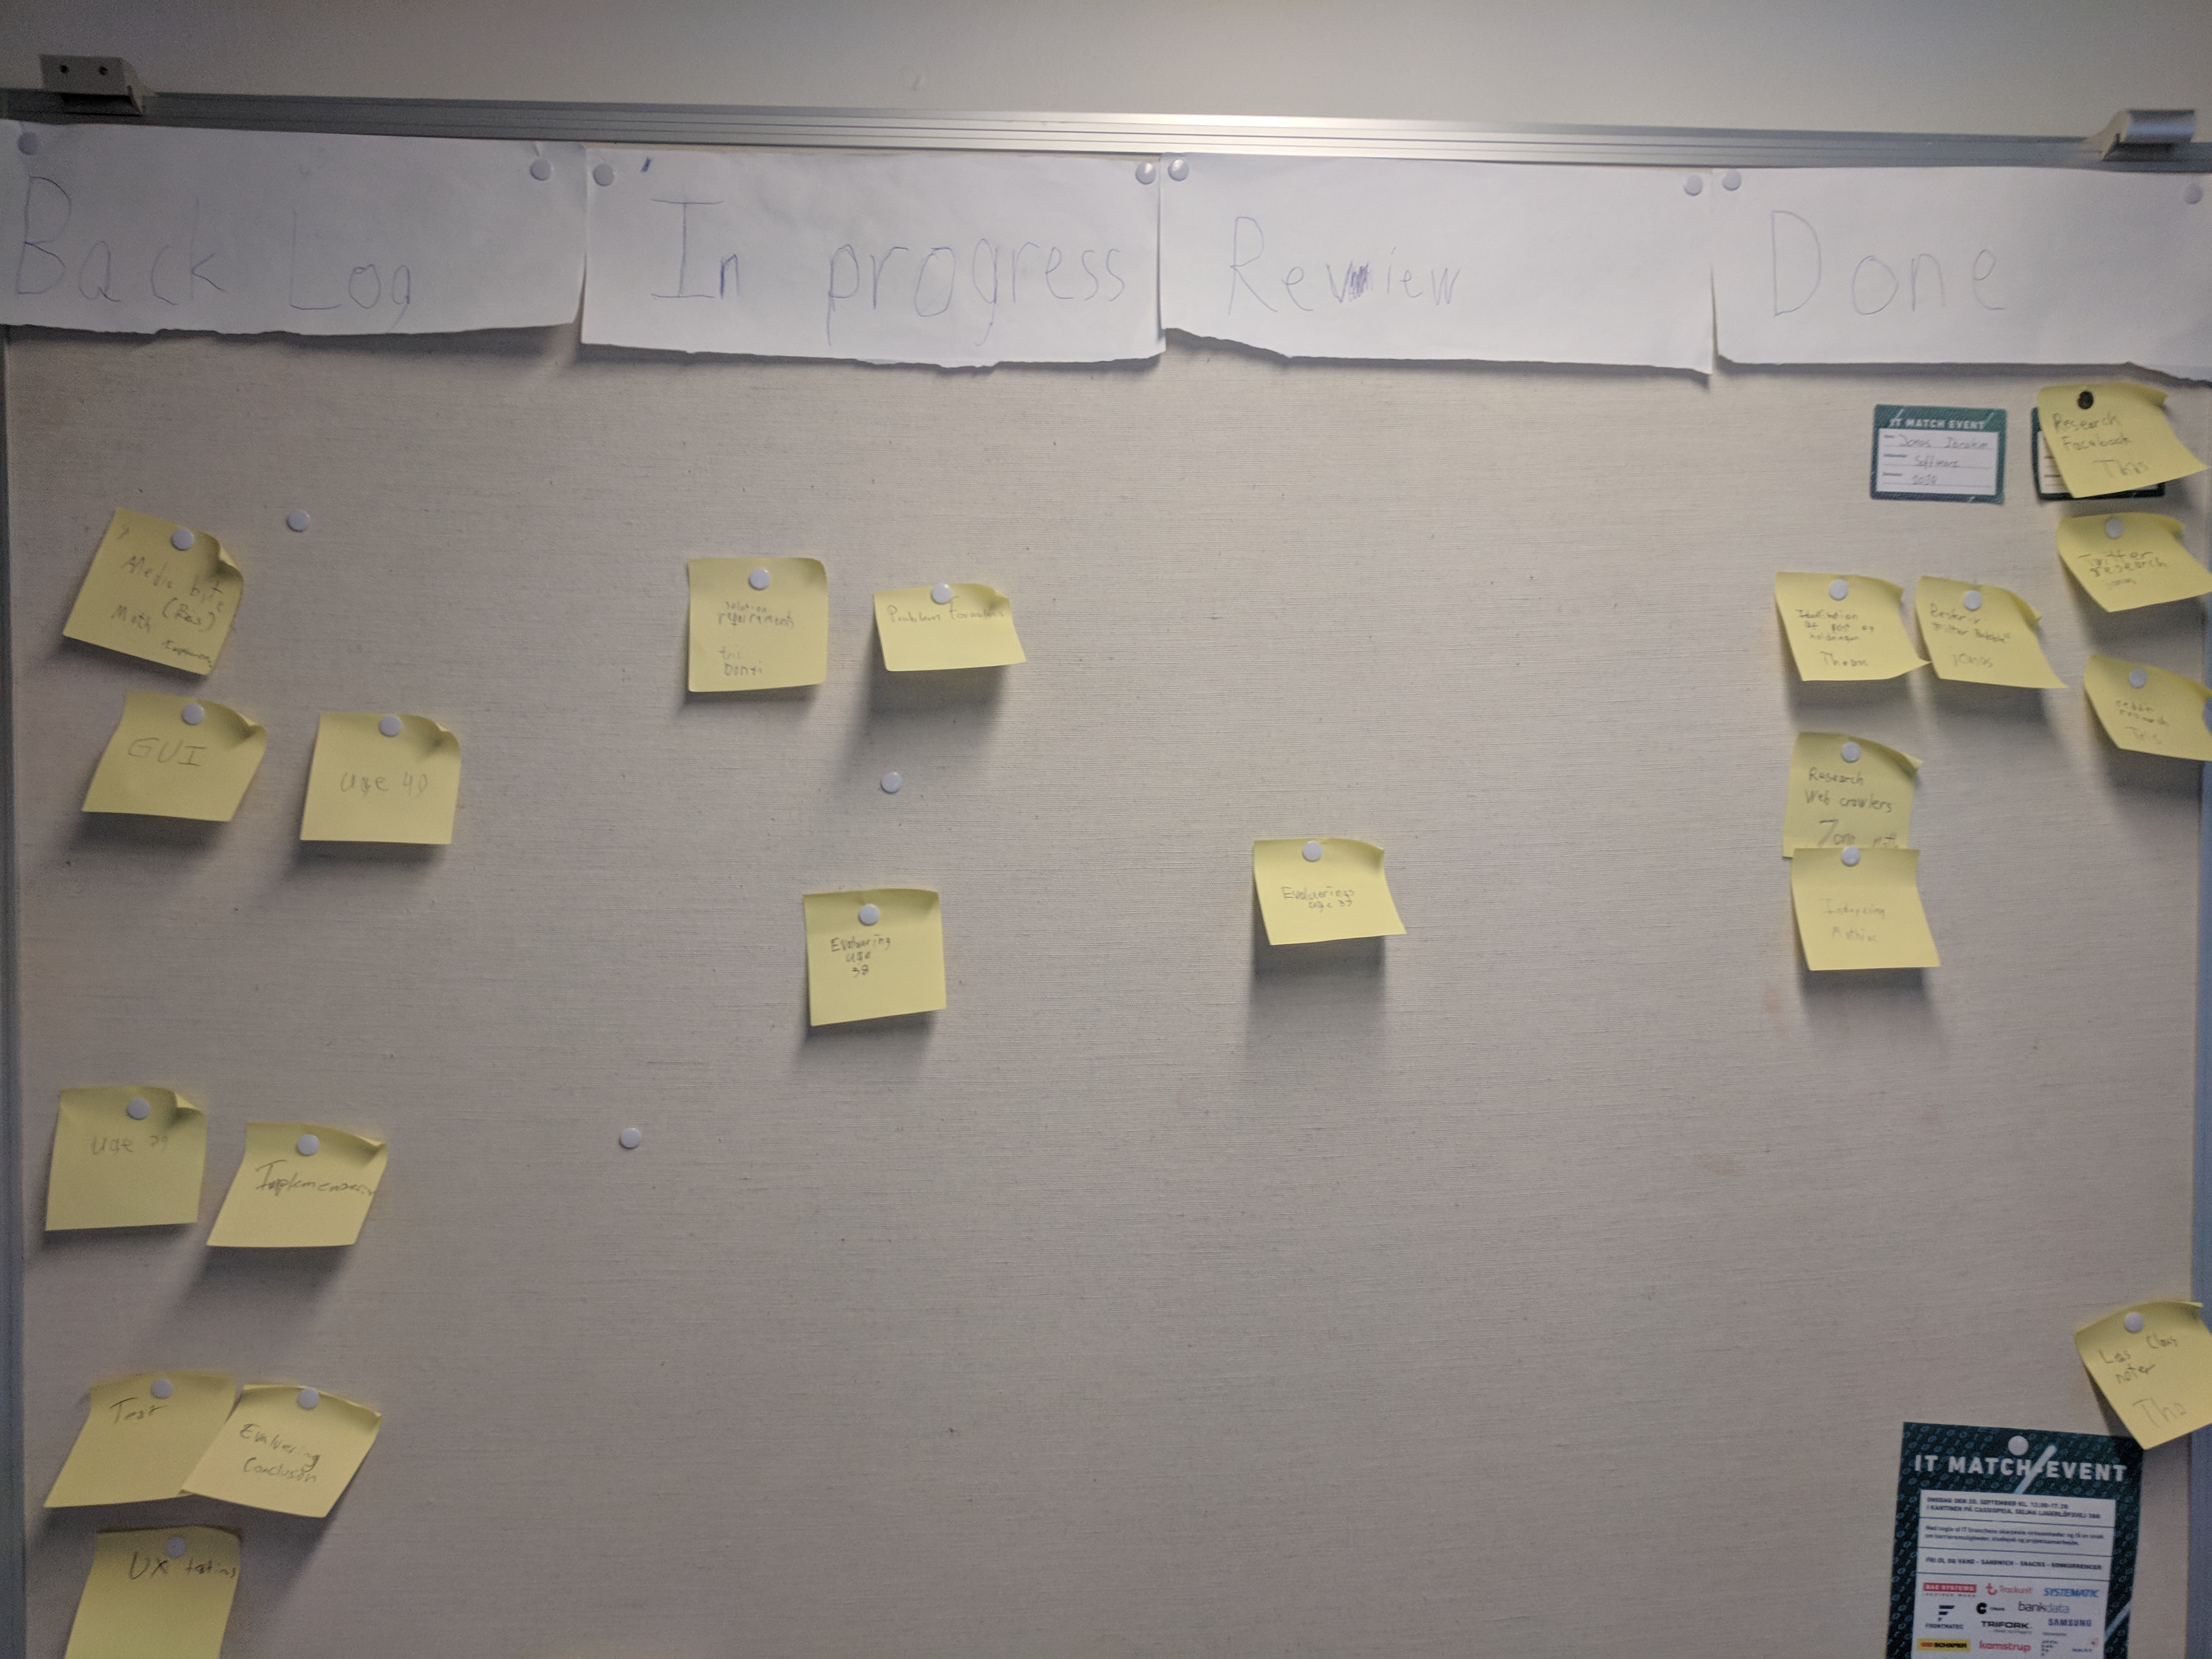
\includegraphics[width =
0.5\textwidth]{figures/Board.jpg}
	\caption{Our board SCRUM element.}
\end{figure}]

\subsection*{Reflection}
We had narrowed us down with the social media sites to the ones we thought were
best, therfore we investiated further and found many we had not considered. The
report is progressing but getting updates as we learn new stuff, perhaps we
should have studied some of the topics further to avoid much rewriting in the
analysis part. There are not many gaps in our schedule for project work this
semester, with all the lectures.

We have made some plans to improve the group's structure and workflow. We made a
short description of the final product, but it was mainly for the supervisor to
see, and it will definitely be updated after. We also look forward to seeing how
morning meetings will help with information sharing.

We found that Facebook is a very restrictive media, with its user-data, and does
not part with information easily. We would have to ask for permission to crawl
Facebook, and from the limited amount of crawlers permitted to do so, then it is
unlikely that we will get the chance. Therefore we are starting to look further into
Twitter and Reddit, as a source for user data, on the initial lookup Twitter's
data looks accessible.

\subsection*{Next Week}
During the next week we want to finish the parts of the report in editing, and
get the rest of the analysis into the editing phase. We would also like to get
started on the data gahtering part of the report. Nedxt week will have focus on
indexing the sites crawled, which means we hope that we are able to see the data
we will be working with.







% Facebook is restrictive, besides that we need to ask for permission. So far we
% are thinking of going in a different direction from facebook. We are looking
% into what is available with twitter and reddit. Alot seems to be available at
% twitter.
% 
% Klaus has had a dat 6 group. We have a degree so we can reach out to companies,
% and we seem more professional. We need a to reflect, and evaluate our UI. We can
% look into books and look for what design process we can follow to develop a UI.
% When we test it should not be a mock-up, but if nothing else provide the
% illusion of depth.
% 
% For reflection, we consider adding a chapter for describing the process.
% 
% We edited the filter bubble and Facebook research parts of the report and
% continued work on the webcrawler.
% Finished research on the links from Klaus, and structured an idea for the final
% webagent.
% Begun on the fundamental request builder to fetch information from Twitter.
% 
% 
% Mail Our Progress:
% We have found that Facebook does not seem to be that great for accurate data.
% We have researched on basic crawlers and its seems like we need permission to
% crawl.
% Twitter and Reddit seem like the best options from our current research.
% 
% The agenda for the meeting:
% 1. Web crawlers and limited access to major social hubs, Facebook doesn't want
% people to crawl their sites. While it seems to be limited on Twitter.
% 2. What do you expect from a 7th semester project? Aside from the semester
% description? 3. How should we document our process? Lone said we needed to
% describe this.
% 
% 
% 
% 
% Here are our notes from today's meeting 
% 
% ---------- Current idea
% for the structure of the rapport:
% Intro (problem description)
% 
% Research Social medial Data gathering Web agent?
% 
% Problem Formulation
% 
% GUI design
% 
% Implementation (done by 25. nov)
% 
% Test User tests Evaluation of the UI Other tests?
% 
% Evaluation
% 
% Rapport:
% Introduction seems good.
% Chapter 2 - Should be more distinctly separated, between formal and reflection.
% Be more concrete about everything, less would, should…
% 
% Discussion:
% Twitter has good possibilities, as we can access a lot of data through their
% API, though we can only make a limited amount of calls every 15 min.
% 
% Thoughts on UI:
% What should the user be shown? Can we find enough info to break the bubble We
% will need to briefly describe the process of designing a GUI but we do not need
% to describe the whole process of iterating through the designs.
% 
% Reflections:
% For the process we can describe some of the difficulties of having all the
% different combination of study. As we need to be better to manage our time. We
% should add our experiences with researching facebook, twitter and reddit and why
% we chose what we chose.

\section*{Week 39}
\subsection*{What Happend This Week}
We created an idea for the structure of the report, and what we wanted in the
chapters. We also set the date 25. November, as the day we would like to be done
with programming. The introduction part is finished, the other analysis chapter
needs to be more coherent.
We have also found that the Twitter \ac{API} gives us access to a vast amount of
user data, although they limit the number of calls we can make every 15 minutes, it
should not cause us any problems. We have made some considerations on the
\ac{UI} of our application. We are starting to consider how much user data we need to break
a filter bubble and if we can get from Twitter.
Our current idea for the semester goal: "We want to help an individual break out
of the filter bubble. The agent checks the user's web activity and provides
information from outside that bubble (how much and what is not finalized yet)."


\subsection*{Reflection}
It was a setback to find out how difficult it was to
get access to social media site's user data through a web crawler. We are now
investigating if there is a way to still use our crawler, we should definitely
have investigated further upon how we could use a crawler instead of its
development.
The Twitter \ac{API} does seem like a suitable option to gather enough user data
about a person, sources explaining that tweets can be used to break the bubble
have been found. Workflow is still a little slower than we liked, we think one
of the problems is that the group only have a full day of work on Mondays. We
learned that we need to be more direct and concise in our report and used too
loose terms such as many "could", "would" and "should".

\subsection*{Next Week}
In an attempt to get more done each week we will try
with a rule, stating that a member meets every day at 9:00 if there is no
lecture for that group member. Next week we want to finish the analysis part of
the report and be able to pull some data from Twitter with the Twitter \ac{API}.



% Our Progress:
%  We have had a busy schedule this week so we don't have much progress to show.
% However, we do have 2 chapters ready for you to read.
%  We have researched further on basic crawlers since it works well with one of
% our courses as well.
%    The agenda for the meeting:
%  1. Feedback on chapters.
%  2. We want to help an individual break out of the filter bubble. The agent
% checks the user's web activity and provides information from outside that
% bubble (how much and what is not finalized yet).

% Research Social medial Data gathering Web agent?  
% Problem Formulation 
% GUI design  
% Implementation (done by 25. nov)  Test User tests Evaluation of
% the UI Other tests?  Evaluation  Rapport:
% Introduction seems good.
% Chapter 2 - Should be more distinctly separated, between formal and
% reflection.
% Be more concrete about everything, less would, should…  Discussion:
% Twitter has good possibilities, as we can access a lot of data through their
% API, though we can only make a limited amount of calls every 15 min.
%  Thoughts on UI:
% What should the user be shown? Can we find enough info to break the bubble We
% will need to briefly describe the process of designing a GUI but we do not
% need to describe the whole process of iterating through the designs.
%  Reflections:
% For the process we can describe some of the difficulties of having all the
% different combination of study. As we need to be better to manage our time. We
% should add our experiences with researching facebook, twitter and reddit and
% why we chose what we chose.
\section*{Week 40}
\subsection*{What Happend This Week}
This week we finished the initial problem and most of the analysis, which is
starting to be near a finishing point. We are now able to retrieve 3200 tweets
from each account a given user is following, meaning that if a user follows five
Twitter accounts then we will find 16000 assuming each account have 3200 tweets
or more.

We have spent some time thinking further upon how to use the vast amount of user
data, we are currently considering focusing on ``emotional wording'' such as
which hashtags and keywords go together, and if it is a positive or negative
tweet.

\subsection*{Reflection}
The application is progressing and we can gather user data now, however, we are
still working on improving the speed. We are not entirely sure about how to
handle the collected data, and we are still researching that. We are wondering
if we fulfil the requirements for the semester, and will discuss what we have
and expect to do and figure out if it is enough with our supervisor. It is
usually a requirement to bring along something from courses and which is
something we need to discuss as well. Our decision to meet at 9:00 is working,
and as a result, the project progress seems to be smoother.

\subsection*{Next Week} 
We will mainly perform edits and improve upon the code
next week because of a Programming Paradigms mini project. Therefore, we do not
expect much more progress.




% Mail
% Our Progress:
% Report: This week we have finished the following sections: Twitter Analysis,
% Initiating Problem and minor corrections (The acronyms in parentheses are marked
% because we haven’t added them properly yet).
% There are still sections in progress, not yet in the master.
% Code: We have managed to retrieve 3200 tweets for each account a given user is
% following. That is, if you follow "denmarkdotdk" and "VisitDenmark", we retrieve
% the 3200 most recent tweets from both of these accounts. We can store this data
% locally, and determine which words and hashtags in the tweets. Now we need to
% determine how we want to analyze the data, and the model we want to use to
% detect the "filter bubble". (We have mostly been talking about a neural network
% which attempts to classify the user's stance on a given subject by using words
% such as "stupid", "amazing", "idiot" etc.) Twitter seems like the best options
% from our current research.
% 
% The agenda for the meeting:
% - It's usually a requirement for us to bring something from our courses, how is
% it this semester? - Feedback

%  regarding the report: I only have minor comments, but rather a major comment
% outside the pdf: in the final report, there will be the scientific part and
% the reflection part (which is also scientific somehow .. ). However, it seems
% to me that in the report, there is also a sort of progress report included a
% bit, which won't be part of the final report. Let's talk about this tomorrow.
%  the code part: sounds exciting. Looking forward to hear more tomorrow.

\section{Reflection on the first part}

Worked on a GUI section (DEB terms), specifically we drew a storyboard and a sketch of the gui.

Reworked text and fixed grammatical errors. Reworked the title in analysis, began on problem statement, and finished working on most of the analysis.

Fixed the threads of the program
We are now able to find the average political value of a bias.

Scheme delivery
\section*{Week 42}
\subsection*{What Happend This Week}
x

\subsection*{Evaluation}


\subsection*{Next Week}





% Our Progress:
% Report: We have restructured the research chapter of the report, and updated
% the problem formulation and it is ready for you to read. We have also
% formulated a list of requirements for our solution which we would like
% feedback on as well.
%  Code: Nothing noteworthy since the last update.
%  The agenda for the meeting:
% 1. Presentation 2. Feedback 3. Which approach would you recommend to analyse
% for the filter bubble data? So far, our data consists of friends, followers,
% tweets (words, hashtags, links, news media). We are unsure of how to best
% analyze this data.
% 4. Should we find live user test the solution with (would most likely be an
% American using Twitter)? 5. A requirement for the project is for our
% application to be internet-application, - agent, or -service. Since we use an
% API for all our Internet-related operations, would you consider this
% requirement as being met?

\section*{Week 43}\label{Week43}
\subsection*{What Happend This Week}
On the report many corrections, some missing introductions and conclusions have
been fixed. From the meeting we found out that we wanted a \ac{GUI} web
application in Laravel \fix{ToDo}{Ref til Laravel} which should connect to a
queue server in C\# through a \ac{REST} \ac{API}. Then the queue should call a
modified version of our workers: program fetching tweets from Twitter. The
\ac{GUI} and workers communicate with a database through another \ac{REST}
\ac{API}. We split all members into different parts and progressed on all,
investigating how and what we should do with them. We quickly found that the
database \ac{REST} \ac{API} should be made in a separate Laravel project.

\subsection*{Evaluation}
During the presentation Monday we received a lot of feedback on everything, and
some keywords or methods extremely useful to us that we had not considered. Such
a presentation meeting is a very useful tool to strengthen a project and
something which should be done in future projects as well. New mini projects for
the complete project that we had not considered before were found through
brainstorming.

\subsection*{Next Week}
During the next week we will continue development on the parts, we have a lot to
do after this meeting. And we will make some considerations on which type of
user we want, university, high school or other? 
The web crawler chapter should be expanded with more information on the \ac{API}
and perhaps some information on why we describe the crawler since we will not
use it.


% All corrections on the report applied and a further grammar check on new
% stuff, introductions and conclusions are also added to the chapters.
%  After the meeting Monday, we discussed how to expand the program we have
% written to be a web application, as such we decided that we need a gui web
% application in Laravel which connects to a queue server in c# through a rest
% api, then the queue server should start workers which are a modified version
% of our first program. The gui and workers communicate with a database though
% another rest api. The rest of the week was spent on trying first to make the
% database rest api in c# but it was then after many problems it was decided
% that the database rest api should be made in a separate Laravel project. Each
% of the for a mentioned items has been worked on during the week.
%   ML-stuff In regards to classifying tweets the week has been spent
% investigating different types of ML, especially Support Vector Machines, Long
% Short Term Memory and basic Neural Networks, which have shown to be promising.
% There has been some thought regarding using different methods for sentiment
% analysis, such as bag of words vs NNs.
%  There has also been devoted time to figuring out whether we should write the
% ML part in python, as it has a lot of good libraries and documentation, or C#
% which has a what appears to be well regarded libraries and somewhat less
% documentation.
%  There has been work on figuring out how to transform tweets into something
% useful, and so far a tweet parser has been built, which transform the tweet
% from a string to a list of string (tokens).
% There has been thought about further transforming the list to a vector by
% mapping words with unique integers, which should be useful when used by a NN.
%  We have considered options for different methods of training, and arrived
% that we are going use the supervised method, though that means we will have to
% provide a lot of tweets which we will have to classify regarding political
% leaning.
%  Meeting:
% Presentation:
% Click on spectrum. Which friends are where.
% Tune what kind og people you want suggested. Very different, slightly
% different from you? Suggest people with a minimum of intellect (University
% degree? Known speaker?) Lookup existing recommendation systems. Current
% systems, reports, solutions? ADs API can maybe group people a bit? Maybe look
% at hashtags? What is our end goal? A plugin? Standalone application? Take
% additional input from the user. What do they think at the moment? What other
% information to supply? Accuracy can partly be determined by user feedback. Do
% you agree with our conclusion? Lookup study about what which hashtags imply
% about a political stance/leaning.
% Look at related work to ours.
% What is the complexity of our algorithm.
% Store information for lookup later.
% Have two approaches system based/neural network. How do they compare? If we
% want to do preprocessing/plugin/(neural network?) we can ask for access to
% (something? computer??)  Meeting:
% Problem with information about reddit user numbers.
% We could "potentially" just write about why our application would be easy to
% scale, and how we would do it  Should we find people to test the application?
% - Maybe, if we can.
%  How do we expand our application:
% - How would we deal with increased popularity - We should probably do
% something with a browser (plugin/site/server/etc.)  What to do:
% - User interface (Laravel) - Describe Architecture MVC front-end. Unknown on
% back-end - Algorithm which uses emotional words, keywords, and hashtags - If
% people log in using their own account, they get an amount of requests for
% themselves - Convert system to run on a server - Definitely do something to
% consider scalability e.g. multiple servers, or using users own requests -
% Begin writing reflections (what should we have done? What did we do? The
% plan?) - Plan how to systematically evaluate our application. User interface,
% testers, usability, functionality (does it work as intended).
% - Look at lecture notes on how to design interfaces. Then do what the slides
% tell us to do.
% - Expand the webcrawler chapter with more info on the different parts of it,
% and in the end a conclusion with the reasonings why we won’t use it (and
% causes like spoofing and a very naughty crawler) - Lookup existing
% recommendation systems. Current systems, reports, solutions?

\section*{Week 44}
\subsection*{What Happend This Week}
We made an early model of a solution including some machine intelligence and
wrote about sentiment analysis. We set-up the database and the \ac{API} for the
database and the authorization for the \ac{API} for the database, and an
implementation part for it in the report Queue server and \ac{REST} \ac{API} for
queues server Setup \ac{GUI} using Laravel and started working on Twitter
authentication.

\subsection*{Evaluation}
We are happy with the direction it is going now, but the workload feels much
harder than before the meeting last week. However, we feel like we are on the
right track, and we talked with our supervisor about getting another meeting
with the expert on a later date. The machine intelligence part seems to be
difficult, and we are running into some problems. Therefore, a person will be
assigned to create an algorithm in case it does not work out as intended.

\subsection*{Next Week} 
Next week we hope to have a better idea about how to classify tweets, and
keep up with progress being made.

% We made an early model of our neural network and wrote about sentiment
% analysis.
%  We setup the database and the API for the database and the authorazation for
% the API for the database, and an implementation part for it in the report 
% Queue server and REST API for queues server  Setup GUI using Laravel and
% started working on twitter authentication  and documentation in the report
% were started for the semester


\section{Reflection on the second part}

The week Nov5-10 in progress
\section*{Week 46} \subsection*{What Happend This Week} 
A feature which retrieves tweets from a set of pre-classified political point of
view (left/right) users, and determines what words they are more likely to use.
This requires a large amount of users with pre-known alignments. To begin, we
have manually compiled a list of Twitter users, which the queue server \ac{API}
now interacts with. The queue server is able to queue jobs for execution. The
queue server instance uses the worker for each job. The worker has been adapted
for use by different threads, such that the limits are not the same for each
thread. We have classified 120 tweets by hand, into 5 classes: Right, little
right, neutral, little left, left.


\subsection*{Reflection} 
We should have started earlier on these weekly summaries and made our notes
better from the beginning, it has caused some mixup and issues doing the clean
writing of them in the report. We have tried to get the same kind of result from
the Naïve Bayes model and algorithm to classify the tweets, this is good since
it permits us to use both or find the one which works best.


\subsection*{Next Week} 
Next week will be slow because of a mini project in Programming Paradigms. Else
everyone has something to work on which will likely not be finished doing that
week.



% We would like feedback on the two weekly summaries, we would like to know if
% the format is fitting.
%   Status:
% We have added a feature to the program which retrieves tweets from a set of
% pre-classified (left/right) users, and determine what words they are more
% likely to use. The idea behind this is, that if we can identify what words are
% most likely to be used by users of specific political alignments, we can
% dynamically update our list of keywords, which we already use for classifying
% users. This, however, requires a large amount of users with pre-known
% alignments. To begin, we have manually compiled a list of twitter users, which
% we use to get started with the word gathering. The idea is, that whenever we
% classify a user with a high degree of certainty, we can add that user to our
% list of users from which we identify words. We have also begun commenting the
% code.
%  The queue server api now interacts with the queue server instance and are
% able to queue jobs for execution. The queue server instance uses the worker
% for each job. The worker has been adapted for use by different threads, such
% that the limits are not the same for each thread.
% Then work began on the section for the queue server api.
%  Did more research into dense feature vectors and other solutions. Found an
% algorithm called word2vec that is interesting.
% With 120 tweets which we have classified by hand, into 5 classes: Right,
% little right, neutral, little left, left. With these tweets we trained a Naive
% Bayesian with bad results, with 5 classes it had a 26% success rate, with 3
% classes it had 44% success. Used a simple SVM with a 3 classes, it had a
% success rate of 30%.
%  Added a TextProcessing Library to the project, which allows us to process
% tweets.
%   As for the agenda:
% We would like feedback on the weekly summaries from the report

\section*{Week 47}
\subsection*{What Happend This Week}
Not much have been done on the project this week, because of our Programming
and Paradigms delivery, however, the following have been done.
Work have been done on weekly summaries, they were not reflective enough which
have been fixed.
Our supervisor helped us setting up another meeting with the expert from week 43
\ref{Week43}, he will listen to what have happend since last and what we plan on
doing and give us feedback. The analysis algorithms have been improved and is
now 8 times faster.

\subsection*{Evaluation}
A major issue has been found when testing the Naive Bayes model. The model
currently predicts that everything belongs in the same category, this should
have been caught earlier perhaps by getting more stats from the test. 
%Kan ikke komme på mere men der burde være andet vi kan refkeltere på

\subsection*{Next Week}
Next week the summaries should be added properly to the report, and
documentation on the different parts of the application should be initiated. The
algorithm and Naive Bayes model should be functioning better and ready for use.


% There haven’t been one much on the project this week because of our Programming
% and Paradigms delivery, however, the following have been done.
% Work have been done on weekly summaries, they weren’t reflective enough which
% have been fixed.
% Our supervisor have also helped us getting a meeting with an expert on the
% field, who will listen to what we plan on doing and give us feedback.
% The analysis algorithms have been improved is is now 8 times faster.
% 
% 
% A major issue has been found when testing the Naive Bayes model. The model
% currently predicts that everything belongs in the same category. We have tried
% to make sure that there is an equal number of cases for each of the outputs,
% though that only changed the prediction to another category.
% 
% We have optimized the analysis algorithm, and improved its runtime by a factor
% of 8. We have also setup the worker such that it can be activated by a call to
% its API. We have also made it possible to post the result to the database
% server.

\section*{Week 48}
\subsection*{What Happend This Week}


\subsection*{Evaluation}


\subsection*{Next Week}



\section{Reflection on the third part}

\section*{Week 49}
This week we made many chages and edits to the report, the initial problem have
also been updated to better fit our current product, and the direction we ended
up taking. We have contacted a person studying politics at Aalborg University to
perform a usertest with, since we wont be able to get a server up and running
with the solution, we will make the test next week.

\subsection*{Reflection}
The weekly reviews are starting to take up much space and becomming many
chapters, it would propably havebeen better to make it a monthly review instead.
Going back and editing them sometimes leads to additions because somethinng took
more than a week and was forgotten when we evaluated on a week. We are not going
to get our product tested on our American demographic \autoref{sec:target}, we
should have considered distribution of our solution earlier, and examined what
we have available at uni. It is part of a learning experience, and we learned a
lot from mistakes which is great. 


\subsection*{Next Week}
We will perform the usability test of our system, we also have a goal of the
report being finished with all additions. Some commenting in the code still
needs to be done, however, no new features will be added. We are starting on the
major editing part and works towards finishing the report for Friday.



% Edits and updates on multiple chapters, initiating problem changed a little to better fit the the context.
% 
% Joanthan
% Fixed mistakes when extracting features, finished the data analysis chapter
% Restructured the analysis part to hopefully provide a better red thread for the reader.
% Began writing the implementation and accuracy testing of the Naive Bayes Implementation.
% 
% DonF
% Test the whole system in action (Not the result GUI screen). Fix some small errors in the code, such as locking the model such that it can be stored by one thread and does not cast the exception that the file is used by another process.
% Helped with collecting test data.
% 
% Mathias
% Made the GUI chapter
% Complete rework of the Worker chapter
% Made the Interaction with Twitter chapter
% A buttload of memes
\section*{Week 50}
During this week we worked hard on finishing the report for Friday, many new
sections and major reconstructions have been performed on the report. The plan
is for everyone to read and comment on the report over the weekend, and finish
it next week. We also had our usability test during a social night, to make it
easier for the person to come by.

\subsection*{Reflection}
We are quiete happy with the progress this week, when it comes to editing then
there is always much reflectionon what could have been better. The usability
test were rushed quiete a bit, we had not entierly tested it on ourselves and
the computer running the system did not have an explanation text to a chapter we
asked her to find, resulting in her being very confused. However, there were
many situations where we could see she had issues, and some questions from her
about decisions. The output from the test was still great and many improvements
happends as a result of it, in the \autoref{cha:usability} describes the test
and what we lerned from it. The raw and premature test was properly not the best
experience from the users point of view, however, it would not be bad to make
the early test with another group. By doing this the flaws and biggest mmistakes
would be removed and hopefully provide a better experience fro the ``non
technical'' user.

\subsection*{Next Week}
During the next week the plan is go through the notes the group created over the
weekend on the report and apply fixes. Since the report wont get anything new
and the code is frozen, then there is no need for a weekly review.


\section{overall reflection}
